\chapter[Online reprocessing simulation]{Online reprocessing simulation}

\section{Online reprocessing method}
The ability to perform online reprocessing of fuel salt improves the potential neutronic performance of liquied-fueled reactors. Firstly, it is unnecessary for liquid-fueled reactors to operate with excess reactivity because fissile material is continuously adding into the core. Secondly, ability to continuously removing fission products that includes strong absorbers (poisons) might significantly improve fuel utilization and decrease neutron leakage. Finally, neutronic parameters could be adjusted ``on-the-fly" without operational cycle interruption. Nevertheless, removal of each element from the liquid fuel salt presents a exclusive problem in terms of storage and disposal of the separated materials.

To take into account online reprocessing two principal approaches might be implemented. One is a batch-wise approach where material is moved into or from the core at specific time intervals (batch). This approach based on assumption that specific material accumulation in the core during the time between separations or feeds does not affect on reactor physics. This method requires the simulation to stop at a given moment in time and restart it with a new fuel salt composition (after removal discharged materials and addition fresh fissile and/or fertile materials). This approach was implemented in a ChemTriton script \cite{powers_new_2013} which has been developed by T.J.Harrision, \gls{ORNL}, and actively using for online reprocessing simulation with SCALE/TRITON \cite{bowman_scale_2011} and Shift \cite{pandya_implementation_2016}. 

Another approach is continuous reprocessing where material is separating from (or added into) the core at all times and exactly simulate a true continuous online reprocessing. This method is more difficult because it requires adding a term to the Bateman equations. In SCALE/TRITON, ORIGEN \cite{gauld_isotopic_2011} solves a set of Bateman equations using one-group averaged fluxes and cross-sections obtained from a transport calculation. Bateman equations that describe the rate of change of the isotopes due to neutron induced reactions and decay
processes could be written in this form \cite{aufiero_extended_2013}:

\begin{align*}
\frac{dN_i}{dt}=\bar{\Phi}\sum\limits_{j}N_{j}\sigma_{j \rightarrow i} - \bar{\Phi}\sum\limits_{j}N_{i}\sigma_{i \rightarrow j} + \sum\limits_{j}N_{j}\lambda_{j}b_{j \rightarrow i} - N_{i}\lambda_{i}
\end{align*}
where $N_i,N_j$ are the number densities of isotopes $i$ and$j$;\\
$\bar{\Phi}$ is averaged in the space and energy spectrum neutron flux;\\
$\sigma_{j \rightarrow i}$ is the microscopic one-group transmutation cross section of nuclide $j$ to nuclide $i$;\\
$\lambda_i$ and $\lambda_j$ are the decay constants of nuclides $i$ and $j$;\\
$b_{j \to i}$ is the branching fraction for neutron absorption by isotope $j$ that lead to the formation of isotope $i$.

The four terms on the right-hand side of the equation represent (1) the production rate of nuclide $i$ from irradiation, (2) the loss rate of nuclide $i$ due to irradiation, (3) the decay rate of nuclide $i$ into nuclide $j$, and (4) the loss rate of nuclide $i$ due to decay. Mentioned earlier deterministic code SCALE/TRITON and Monte Carlo codes MCNP, Shift, KENO-VI does not support non-zero removal or feeds rates for depletion simulations.

Online fuel reprocessing can be explicitly introduced in the system of equations by adding effective decay and transmutation terms for the different nuclides. During fuel composition evolution calculations, the total mass fraction of thorium fluoride is kept constant at 12\%. For this purpose, transmuted into $^{233}$Th isotope are replaced with the fresh $^{232}$Th feed material. It could be achieved by modifying the Bateman equation adding the following additional gain term to the right-hand side:
\begin{align*}
\bar{\Phi}\sum\limits_{k=^{232}Th}N_{k}\sigma_{k,c}
\end{align*}
where $\sigma_{k,c}$ is the one-group capture cross section of thorium-232.

The removal of fission products and protactinium is achieved by adding an explicit decay term to the Bateman equations. For the generic fission product l, following additonal loss term might be added:
\begin{align*}
- N_{l}\lambda_{l,reproc}
\end{align*}
where $\lambda_{l,reproc}$ is the effective removal time constant of the particular chemical specie. This approach was recently implemented as a purpose-made extension of the continuous-energy Monte Carlo reactor physics and burn-up code SERPENT \cite{aufiero_extended_2013} but it is not properly tested and unavailable for ordinary users so far.

To validate and verify in the nearest future the SERPENT 2 online reprocessing capability, I have been developed Python-based script, Saltproc, implementing batch-wise approach on the top of SERPENT 2 burnup routine. High-fidelity full-core \gls{MSBR} model serves as a benchmark in online reprocessing simulation described in this thesis. Assessment against the SERPENT 2 continuous online reprocessing procedure based on the benchmark is not treated here.

The \gls{MSBR} has the capability to remove all poisons (e.g. $^{135}$Xe), noble metals, and gases (e.g. $^{75}$Se, $^{85}$Kr) every 20 seconds. The $^{232}$Th in the fuel absorbs thermal neutrons and produces $^{233}$Pa which then decays into the fissile $^{233}$U. Protactinium presents a challenge, since it has a large absorption cross section in the thermal energy spectrum. Accordingly, $^{233}$Pa is continuously removed from the fuel salt into a protactinium decay tank and allowing $^{233}$Pa to decay to $^{233}$U without poisoning the reactor. The reactor reprocessing system is designed to separate $^{233}$Pa from the molten-salt fuel over 3 days, hold it while $^{233}$Pa decays into $^{233}$U, and return it back to the primary loop. This feature allows the reactor to avoid neutron losses to protactinium, keeps fission products to a very low level, and 
increases the efficiency of $^{233}$U breeding. Principal scheme of \gls{MSBR} reprocessing facility has shown on figure~\ref{fig:material_flow}. Table~\ref{tab:reprocessing_list} summarizes full list of nuclides and the cycle times used for modeling salt treatment and separations \cite{robertson_conceptual_1971}. 

%%%%%%%%%%%%%%%%%%%%%%%%%%%%%%%%%%%%%%%%
\begin{table}[ht!]
        \centering
        \caption{The effective cycle times for protactinium and fission product removal \cite{robertson_conceptual_1971}.}
        \begin{tabular}{|m{0.25\textwidth} | m{0.45\textwidth}|m{0.20\textwidth}|}
        \hline 
        %\begin{tabularx}{\linewidth}{l X} \toprule 
        Processing group & \qquad Nuclides & Cycle time (at full power) \\ [5pt] \hline 
        Rare earths & Y, La, Ce, Pr, Nd, Pm, Sm, Gd & 50 days \\ [5pt] \hline 
        \qquad & Eu & 500 days \\ [5pt] \hline
        Noble metals & Se, Nb, Mo, Tc, Ru, Rh, Pd, Ag, Sb, Te & 20 sec \\ [5pt] \hline
        Seminoble metals & Zr, Cd, In, Sn & 200 days \\ [5pt] \hline
        Gases & Kr, Xe & 20 sec \\ [5pt] \hline
        Volatile fluorides & Br, I & 60 days \\ [5pt] \hline
        Discard & Rb, Sr, Cs, Ba & 3435 days \\ [5pt] \hline
        Salt discard & Th, Li, Be, F & 3435 days \\ [5pt] \hline
        Protactinium & $^{233}$Pa & 3435 days \\ [5pt] \hline
        Higher nuclides & $^{237}$Np, $^{242}$Pu & 16 years \\ [5pt] \hline
        \end{tabular}
        \label{tab:reprocessing_list}
          \vspace{-0.9em}
\end{table}
Since removal rates vary among nuclides in this reactor concept, the SERPENT 2 build-in reprocessing subroutine is unable to capture the desired reprocessing strategy. The removal rates also dictate the necessary resolution of depletion 
calculations. If the depletion time intervals are very short an enormous number of depletion steps are required to obtain the equilibrium composition. On the other hand, if the depletion  calculation time interval is too long, serious impacts of short lived fission products are not captured in a manner that is faithful \gls{MSBR} conceptual design. To compromise, the time interval for depletion calculations in this model was selected as 3 days to correlate with the removal interval of $^{233}$Pa and thorium was continuously added to maintain the initial mass fraction of $^{232}$ThF$_4$.

\begin{figure}[htp!] % replace 't' with 'b' to 
  \centering
  \vspace{-0.3em}
  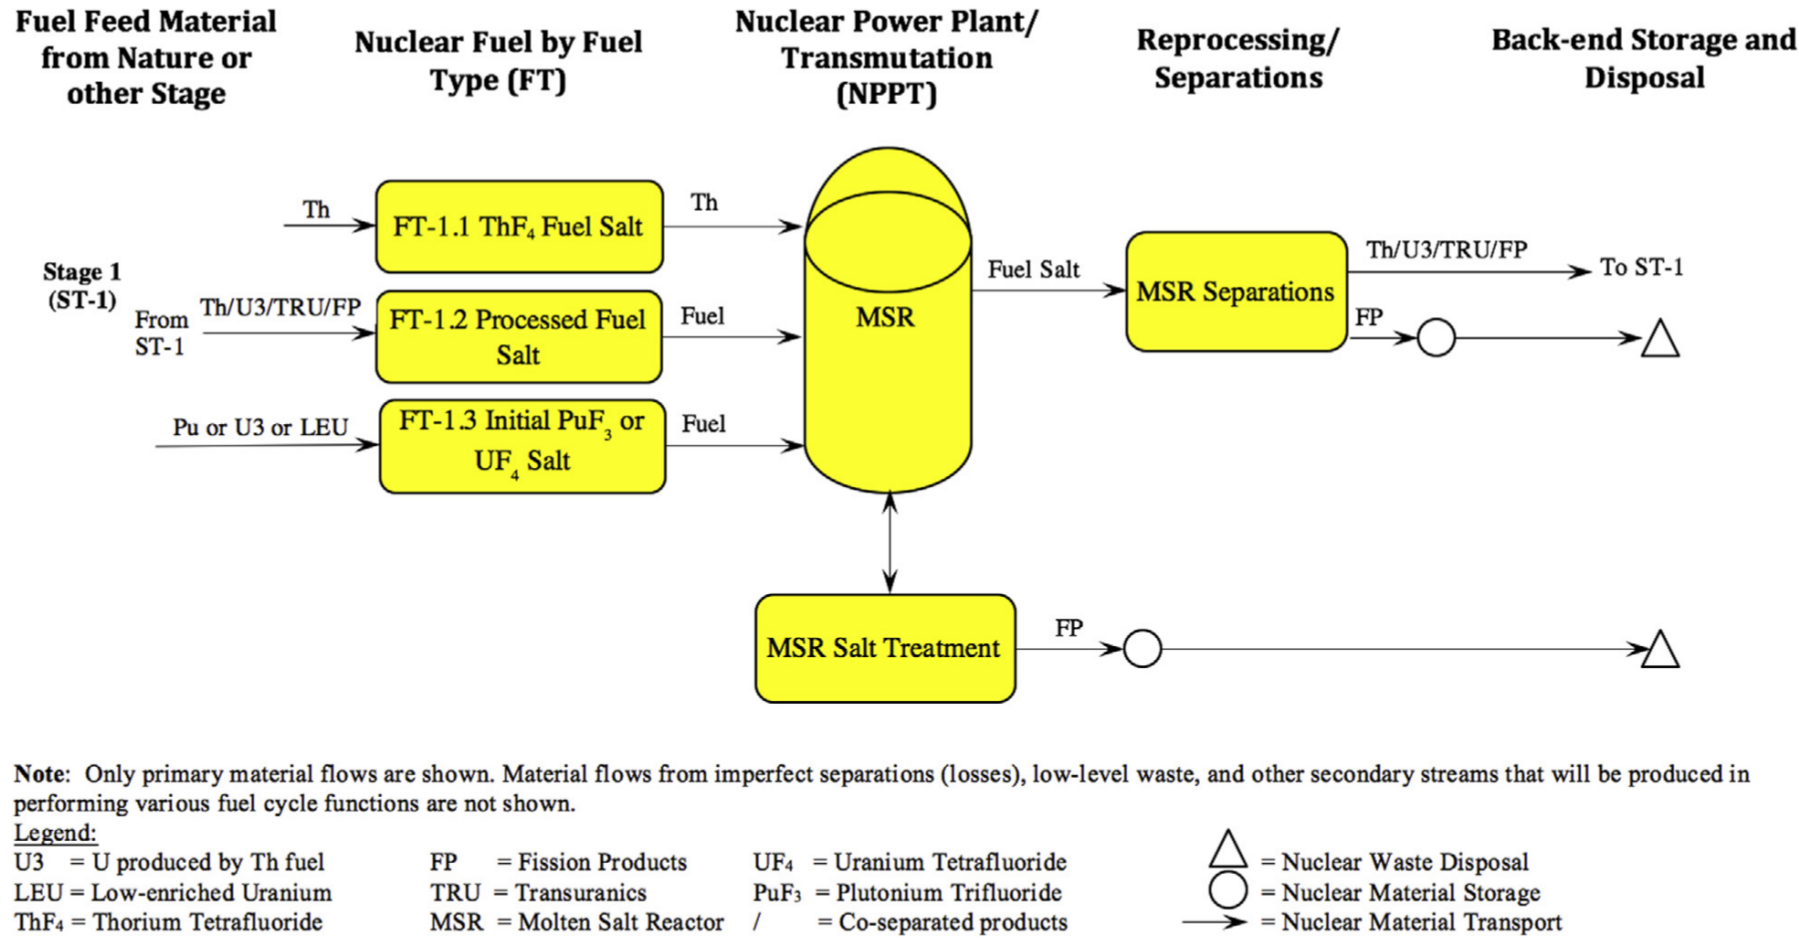
\includegraphics[width=\textwidth]{material_flow_dia.png}
  \caption{The material flow diagram for the single-stage \gls{MSR} fuel cycle showing a first stream (FT-1.1) that represents the fissile and fertile material load at startup \cite{wigeland_nuclear_2014}.}
  \vspace{-0.6em}
  \label{fig:material_flow}
\end{figure}
\FloatBarrier

\subsection{Simplifying assumptions}
The main goal of present study is to identify the effects of moving materials from and to the reactor core, and find equilibrium performance of a thorium fuel cycle using \gls{MSBR}. To highlight these effects and simplify the analyses, several assumptions have been made.

\section{Python code description}

\section{Results and equilibrium state analysis}